\subsubsection{Recirculation algorithm}
\label{sec:models-recirc} 

The \emph{Recirculation algorithm} designed by \citet{hinton1988learning} is an unsupervised neural letwork for learning encoder tasks. Motivation for such a model comes from interesting hidden representations of Backpropagation (\ref{sec:models-bp}) with possible usage as an encoder. It has only two layers denoted \emph{visible layer} and \emph{hidden layer} as shown on figure~\ref{fig:models-recirc}. The aim of the network is to remember on the hidden layer the patterns presented to the visible layer. This could be used for compression if the hidden layer has less units than the visible layer. It also could be used as a content--accessed--memory where if novel patterns are presented to the network it could show the most similar stored pattern. 

\begin{figure}[H]
  \centering
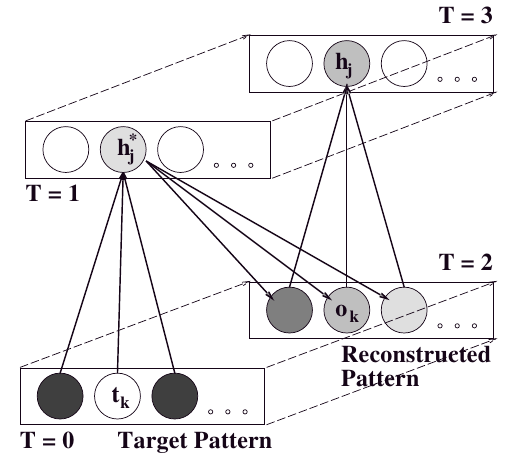
\includegraphics[width=0.4\textwidth]{img/recirculation.png}
  \caption{The recirculation algorithm by \citet{hinton1988learning}. }
  \label{fig:models-recirc}
\end{figure}

As depicted on \ref{fig:models-recirc} activation is propagated in four steps $T \in \{0,1,2,3\}$. At the first phase denoted by $T=0$ only the input vector $t$ is clamped on the visible layer, at $T=1$ a forward pass $h^{*}$ is computed from visible to hidden, at $T=2$ a reconstructed pattern $o_k$ as a function of hidden state $h^{*}$ at $T=1$ is computed and finally at $T=3$ a hidden state $h$ is computed from $o_k$.

For the reconstruction to work \emph{symmetric} weights are used. The learning rule is common for both visible and hidden layers and it;s based only on difference of activations: 
\begin{align}
\frac{\partial E}{\partial w_{ij}} &= -(\eta^{*}_j - \eta_j) \phi'(\eta_j) t_k \nonumber \\
&\approx -(h^{*}_j - h_j)t_k \nonumber 
\end{align} 
The approximation step could be made because $\phi'(\eta_j)$ has \emph{usually} same sign as $(\eta^{*}_j - \eta_j) $ \citep{hinton1988learning, o1996bio}. The approximation works better if the difference of activations is smaller and therefore the activation for the reconstructed pattern $o$  is made similar to target pattern $t$: 
\begin{equation}
o_k = \alpha t_k + (1-\alpha)f(\eta_k). 
\end{equation} 

%Authors study the case of asymetric weights. They do not provide a proof of convergence but they provide some intutition why it should work. Also they link the work of Ballard who experimented with connecting (merging) several closed loops so that hidden units of closed loops can be input units of other closed loops of recirculation.

%\paragraph{From the original article.}
%Instead of using a separate group of units for the input and output we use the very same group of \textit{visible} units, so the input vector is the initial state of this group and the output vector is the state after information has passed around the loop. The difference between the activity of a visible unit before and after sending activity around the loop is the derivative of the squared reconstruction error \citet{hinton1988learning}.

%On the first pass, the original visible vector is passed around the loop, and on the second pass ana average of the original vector and the reconstructed vector is passed around the loop. The learning procedure changes each weight by an amount proportional to the product of the \textit{presynaptic} activity and the \textit{difference} in the post-synaptic activity on the two passes  \citet{hinton1988learning}.

